\documentclass[12pt,a4paper,oneside, titlepage]{report}

\usepackage{times}
\usepackage[frenchb]{babel}
\usepackage{hyperref} 
\usepackage[utf8]{inputenc}
%\usepackage[T1]{fontenc}
%\usepackage{amsmath}
%\usepackage{amsfonts}
%\usepackage{amscd}
%\usepackage{amstext}
%\usepackage{amssymb}
%\usepackage{bar}
\usepackage{color}
%\usepackage{mathrsfs}
\usepackage{graphicx}
%\usepackage{calligra}
%\usepackage{amsthm}
%\usepackage{multirow}
%\usepackage{tabularx}
%\usepackage{layout}
%\pagestyle{headings}
\usepackage{fancyhdr}
\pagestyle{fancy}

%\setlength{\textheight}{630pt}
%\setlength{\footskip}{30pt}
\newtheorem{defi}{D\'efinition}[section]
\newtheorem{note}{Note}[section]
\newtheorem{proprietet}{Propri\'et\'e}[section]
\newtheorem{exemple}{Exemple}[section]
\newtheorem{corollaire}{Corollaire}[section]
\newtheorem{rem}{Remarque}[section]
\newtheorem{thm}{Th\'eor\`eme}[section]
\newtheorem{illustration}{Illustration}[section]
\newenvironment{demonstration}{\begin{proof}[\textnormal{\textbf{Preuve.}}]}{\end{proof}}
\definecolor{gris}{gray}{0.45}
\setlength{\parindent}{1cm}
\newcommand{\textcalli}[1]{{\small{\textbf{$\negmedspace$\calligra #1}}}}

\renewcommand{\chaptermark}[1]{\markright{\thechapter\ #1}}
%\renewcommand{\sectionmark}[1]{\markright{\thesection\ #1}}
\fancyhf{} % supprime les en-têtes et pieds prédéfinis
\fancyhead[R]{\thepage}% Left Even, Right Odd
\fancyhead[L]{\textsl{\leftmark}} % Left Odd
%\fancyhead[RE]{\textsl{\leftmark}} % Right Even
\renewcommand{\headrulewidth}{0pt}% filet en haut de page
\renewcommand{\footrulewidth}{0pt} % pas de filet en bas
\fancypagestyle{plain}{ % pages de tetes de chapitre
\fancyhead{} % supprime l’entete
\fancyhead[R]{\thepage}
\renewcommand{\headrulewidth}{0pt} % et le filet
}

\begin{document}

%newpage
%\thispagestyle{empty}
%\null
%\newpage
\pagenumbering{roman}
\chapter*{Remerciements}
\renewcommand{\leftmark}{REMERCIEMENTS}
%\addcontentsline{toc}{chapter}{Remerciements}

Nous remercions ...\\

\newpage
\renewcommand{\leftmark}{TABLE DES MATI\`{E}RES}
\thispagestyle{fancy}
\tableofcontents


\newpage
\pagenumbering{arabic}
\renewcommand{\leftmark}{INTRODUCTION}

\chapter*{Introduction}

L'avènement de L'$Internet$ $of$ $Things$ a lancé une nouvelle ère d'appareils connectés, ouvrant de nouvelles possibilités de partage de l'information, d'automatisation et de protection. Bien que le concept lui même soit prometteur, la technologie qui l'accompagne est essentielle.

Les premières technoligies utilisées pour l'IoT étaient les technologies sans fil déja présentes comme le Wifi ou le Bluetooth. Performantes dans certains cas, elles étaient néanmoins limitées : une consommation en énergie élevée, une portée restreinte et parfois même un cout d'infractrucutre trop important.

Dans ces circonstance est apparu $LoRa$, une technologie développée en particulier pour l'IoT. Sa capacité à gérer les communications longue portée même dans des environements peu adaptés est une révolution pour le domaine.

L'expansion de L'Iot soulève une nouvelle problèmatique de sécurité. Entre autres, l'indentification des noeuds au sein des réseaux est essentielle. Il a été découvert que des noeuds fabriqués avec les mêmes microprocesseurs et modèles d'émetteur-récepteur radio peuvent présenter de subtiles particularités dans les caractéristiques de leurs signaux. Cette variabilité intrinsèque de la transmission des signaux radio peuvent être exploitées pour distinguer les noeuds d’un réseau. En écoutant leurs signaux radio émis et en analysant leurs signatures distinctes, il devient possible de les identifier.

Ce travail est structuré en trois parties. Le premier chapitre sert d'aperçu global du signal radio afin d'y développer et rappeler les concept de télécommunication de base. Ce chaptire présente également les technologies LoRa et LoRaWAN à travers leurs caractéristiques et leur pertinence dans l'IoT.

Le second chapitre est dédié à l'étude expérimental du sujet. Les aspect pratique y seront appliqués, notamment l'utilisation de radio logicielle afin de capturer des signaux radio. Ces signaux seront ensuite analysé grace à diverse méthodes détaillé dans ce chapitre.

La dernière partie du travail présentera une présentation des résultats obtenu en suivant l'analyse effectuée au chapitre précédant. Enfin le travail sera achevé en concluant sur de potentielle implications plus larges à ce sujet ainsi que des recherches plus approfondies.

\chapter{Rappels et nomination des technologies}

\section{signal radio}

Un signal est une variation dans l'espace ou dans le temps d'une quantité physique contenant de l'informations. Un signal peut être continu ou discret, on le nomme alors respectivement analogique ou numérique. Le type de signal dépent notamment de l'information qu'il contient. Un signal analogique peut contenir par exemple du son, là où un signal numérique contient généralement un nombre fini de valeur (par exemple des 0 et 1).
Les deux catégories ne sont pas incompatible car il est souvent nécessaire en télécommication de pouvoir passer de l'un à l'autre.

L'utilisation de signaux radio en télécomunication confère de nombreux avanages, comme la portée, la vitesse de transmisison , la résistance aux interférence ou encore le coût de propagation. Tout ces avantages sont possible car un signal peut être modulé. La modulation est un technique permettant de modifier les propriétés du signal lui permettant de transporter de l'information.

En télécommunication, les signaux sont associés aux ondes radios, ainsi appelé $radio signal$ ou signal radio. Voici les principals attributs d'un signal radio: 

\begin{itemize}

\item la frécquence, mesurée en Hertz. Elle détermine le combre de cycle qu'accomplie le signal par seconde.
\item La largeur de spectre, elle dépent de la fréquence car c'est l'écart entre la plus haute fréquence et la plus basse du signal. Une plus grande parleur permets de transmettre plus d'information.
\item L'amplitude. Selon le type de signal l'attribut possède différentes fonctions. Dans le cas d'un signal analogique l'amplitude est l'une des caractéristique principale d'identification du signal mesurant l'ampleur du signal. dans un signal numérique l'amplitude set plutot demarge entre les différentes états du signal. 
\item la puissance, mesurée en décibel (dB). C'est la force du signal, un attribut important pour la réception du signal notamment.
\item le $signal$ $to$ $noise$ $ratio$ ou SNR. Cet attribut mesure la qualité du du signal. une valeur élevée indique que le pourcentage de bruit est faible.
\item le $bit$ $rate$,ou le taux de transmission mesure la quantité de donnée transmise en bit par seconde. cet attribut est exclusif aux signaux numériques. On parle de $Baud$ $rate$ pour les signaux analogiques. Ce n'est pas excatement l'équivalent du bit rate car c'est le nombre de symbole modifié par seconde, et un symbole peut contenir plusieurs bit pour un signal numérique.

\end{itemize}

\section{traitement du signal}

\subsubsection{modulation}

La réception d'un signal nécessite des antennes dont les dimensions dépendent de la longueur d'onde du signal. un signal a haute fréquence à l'avantage d'être facilement transmissible sur une grand portée. Cependant les signaux originaux appelé $baseband$ $signal$ sont en basse fréquence. La modulation d'un signal permet de transformer le signal en haute fréquence, devenant ainsi le signal modulé.

Parmis ces différents attributs, certains sont utilisés pour effectuer une modulation. Les deux modulations les plus utilisés sont basées sur les attributs de la frécquence et de l'amplitude. La modulation en fréquence (ou $FM$ pour $frequency$ $modulation$) consiste à encoder l'information en faisant varier la frécquence en maitenant l'amplitude constance. La modulation en amplitude ($AM$) est le procédé inverse, c'est à dire encoder l'information en faisant varier l'amplitude tout en gardant la fréquence constante. 


La modulation en amplitude est plus ancienne et est encore utilisé dans beaucoup de systèmes. Cette technique possède moins de contrainte car elle plus simple à implémenter. Elle requiert le signal modulant et un signal haute fréquence appelé $carrier$  $signal$

Soient un signal modulant $u(t)$ et un sigal porteur (ou $carrier$ $signal$) $v(t)$, la modulation en fréquence s'effectue en multipliant les deux signaux pour obtenir le signal modulé $s(t)$ = $u(t)$ . $v(t)$

\begin{figure}[h]
\centering

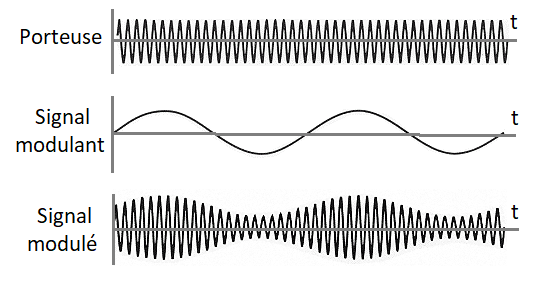
\includegraphics[scale=1]{../images/AM_mod.PNG}
\caption{Exemple de modulation en amplitude}\label{term4}
\end{figure}


La modulation en fréquence permet d'obtenir des transmission de meilleur qualité plus résistante à leur environement tout en gardent une puissance d'émission constante. 

Soient un signal modulant $u(t)$ et un signal porteur sinuosidal $v_{p}(t)$ = $A_{p}cos(2\pi f_{p}t)$ où

$f_{p}$ est la fréquence de la porteuse,
$A_{p}$ est l'amplitude de la porteuse,

alors le signal modulé $s(t)$ = $A_{p}cos(2\pi \int_{0}^{t}f(\tau)d\tau)$ où

$f$ est la fréquence instantanée. Elle s'exprime en fonction de la dérivation de fréquence $f_{\Delta}$, c'est à dire la dérivation maximale par rapport à la fréquence de la porteuse $f_{p}$. $f(t)$ = $f_{p}$ + $f_{\Delta} u(t)$

\begin{figure}[h]
\centering

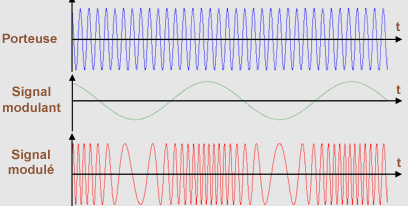
\includegraphics[scale=1]{../images/FM_mod.PNG}
\caption{Exemple de modulation en fréquence}\label{term4}
\end{figure}



\subsubsection{gestion du bruit}



L'un des attributs cités concerne le bruit. Un signal est toujours affecté de petites fluctuations plus ou moins importantes, et sont les origines peuvent être diverses. Ces perturbations, appelée $bruit$ en télécommunication se définissent par l'altération non souhaité de l'intégrité d'un signal. Le bruit peut prendre différente formes, des perturbations de type essentiellement impulsionnel engendrées par des commutations de courants ou alors du bruit de fond généré dans les câbles et les composants électroniques en raison
des mécanismes statistiques de la conduction électrique. Il est possible de réduire voir élimier l'influence des perturbations impulsionelles. En revanche, le bruit de fond est lui irreductible. Tout signal sans bruit n'existe pas, même à l'emission. Il est cependant possible que le bruit devienne invisible si son niveau est très faible. L'attribut SNR est donc un critère de la qualité du signal.


\subsubsection{transformée de Fourier}

Pour effectuer une analyse de signal, sa représentation est capitale. Les Figure 1 et 2 représente des signaux en fonction du temps écoulé. Il est possible de représenter des signaux selon une autre composante, la fréquence.


La transformée de Fourier est un outil fondamental utilisé pour analyser et décomposer des signaux complexes en composantes fréquentielles. En transformant un signal dans le domaine temporel en sa représentation dans le domaine fréquentiel, la transformée de Fourier révèle les différentes composantes fréquentielles présentes dans le signal. En fonction du type de signal, la transformée de Fourier est adaptée.

Pour les signaux continus, la $CFT$ (Transformée de Fourier continue) convertit une fonction du temps en fonction de la fréquence en intégrant le signal par rapport aux sinusoïdes de toutes les fréquences possibles. Cette transformation fournit les informations d'amplitude et de phase pour chaque composante de fréquence présente dans le signal.

pour les signaux discrets et échantillonnés, la DFT (Transformée de Fourier discrète) calcule un ensemble fini de composantes de fréquence. Il est calculé à l’aide d’un nombre fini d’échantillons, ce qui donne des composantes de fréquence discrètes. Il existe un méthode simplifiée pour les signaux discret appelé FFT (Fast Fourier Transform). Il s'agit d'un moyen plus rapide de calculer la transformée de Fourier, en particulier pour les signaux numériques comportant un grand nombre de points de données. L'avantage principal de cet algorithme permet de réduire le temps de calcul en divisant la DFT en sous problèmes. La FFT est une méthode très utilisée pour l'analyse de signaux.

\newpage

\section{LoRa}

$LoRa$ (Long Range) est une technologie de communication sans fil qui permet de transmettre des données sur de longues distances avec une faible consommation d'énergie. Elle a été développée par la société française Cycleo et est maintenant gérée par la fondation LoRa Alliance, qui regroupe plusieurs entreprises et organisations du monde entier.

LoRa est principalement utilisée dans l'$Iot$. Elle se distingue par sa portée étendue, qui peut atteindre plusieurs kilomètres en milieu urbain et plusieurs dizaines de kilomètres en milieu rural, ainsi que par sa faible consommation d'énergie, qui permet de prolonger la durée de vie des appareils connectés. Une longue portée avec un puissance limitée induit une plus faible bande passante que les autres technologies sans fil (le Wifi, la 4G, Bluetooth etc).


LoRa utilise une bande de fréquences qui varie selon les régions du monde où LoRa est déployée :
\begin{itemize}
\item en Europe, la bande de fréquences autorisée est comprise entre 863 et 870 MHz,
\item aux États-Unis, elle se situe entre 902 et 928 MHz,
\item en Chine, la fréquence autorisée varie entre 779 et 787 MHz,
\item les régions restantes ont elles aussi une fourchette unique.
\end{itemize}

La technologie LoRa utilise la modulation en fréquence chirp spread spectrum (CSS). la modulation CSS utilise un signal chirp, c'est à dire un signal modulé en fréquence linéaire. Ce signal a une amplitude constante mais balaie tout le spectre de la bande passante de manière liénaire dans une période de temps définie. Cette technique de modulation sera détaillé plus loin dans le chapitre.

La technologie LoRa utilise également une technique de multiplexage en temps partagé (TDMA) pour permettre à plusieurs appareils de partager la même bande de fréquences de manière à maximiser l'utilisation de la capacité de transmission. Elle utilise également une technique de diffusion de données (multicast) pour envoyer les mêmes données à plusieurs appareils simultanément, ce qui permet de réaliser des économies de bande passante et d'énergie.

En plus de sa portée étendue et de sa faible consommation d'énergie, LoRa se distingue par sa sécurité de transmission, qui est assurée grâce à l'utilisation de codes de sécurité uniques et à la possibilité de chiffrer les données transmises. Elle est également compatible avec de nombreux protocoles de communication couramment utilisés dans l'IoT, tels que TCP/IP, HTTP et MQTT, ce qui facilite son intégration dans les systèmes existants.

Toutes ces  particularités font de LoRa une technologie complémentaire à celles déja existente plutot que rivale.

LoRa se compose de deux éléments principaux : la couche physique de la technologie et LoRaWAN, la couche MAC (media access control), une sous couche de la couche liaison de données. la couche physique de LoRa gère la fréquence radio ainsi que la modulation. LoRaWAN gère les aspects réseau (sécurité, propagation, adressage et sécurité).

\subsection{couche physique LoRa}

\subsubsection{découpage de la couche physique}

Les étapes de la conception de la couche physique de LoRa sont les suivantes :
\begin{itemize}
\item Le codage de canal est une technique utilisée dans les systèmes de communication sans fil pour améliorer la robustesse et la fiabilité de la transmission des données. Dans le cas de LoRa, le codage de canal est une étape importante pour s'assurer que les données transmises sont correctement reçues et décodées par le récepteur en utilisant de la redondance.
\item Le mélange de canal (en anglais "channel interleaving") est la dernirèe des méthode d'amélioration de la robustesse de la tranmission des données. 
Cette technique consiste à réarranger les données avant de les transmettre, en les intercalant entre elles de manière à les disperser sur le spectre des fréquences de la transmission. Cela permet de réduire l'impact des erreurs de transmission sur la qualité de la réception, en évitant que des erreurs consécutives ne se propagent et ne perturbent la décodage des données.
\item Le blanchiment de canal (en anglais "channel whitening") est une méthode d'amélioration de la robustesse et de fiabilité de la transmission des données. Le blanchiment de canal est également une étape importante pour s'assurer que les données transmises sont correctement reçues et décodées par le récepteur.
Cette technique consiste à utiliser une transformation aléatoire ou pseudo-aléatoire des données avant de les transmettre, de manière à répartir le spectre des fréquences de la transmission sur une large gamme de fréquences. Cela permet d'obtenir une meilleure résistance aux interférences et aux bruit de fond, ainsi qu'une meilleure robustesse face aux erreurs de transmission. En effet la transformation de la séquence assure une corrélation faible entre les bits de cette dernière.
\item La modulation CSS est l'étape la plus importante pour le sujet de ce travail. En effet, le signal modulé permet d'obtenir une séquence de $chirp$ ou un signal $chirp$. Cette séquence est unique et permettrait l'identification du noeud éméteur. 
\item demodulation CSS
\item dewhitening
\item deineterleaving
\item decoding
\end{itemize}


Cette analyse a été faite en $reverse engeneering$. Le reverse engineering consiste à analyser un produit ou un système afin de comprendre comment il fonctionne ou d'identifier ses principes de conception. Dans le contexte de LoRa, le reverse engineering examine la technologie derrière LoRa afin de comprendre ses principes de base et sa conception.

\subsubsection{modulation CSS}

principe de base : the signal est modulé en sweepant sur un large bande de fréquence en utilisant des signaux "chirp". deux type de chirp "upchirp" et "downchirp".

upchirp : la fréquence augmente avec le temps
downchirp: la fréquence diminue avec le temps

le signal est séparé sur une large bande de fréquence, permettant par exmeple plusieurs transmission sans causer d'interférence. la modulation CSS étale sur une bande plus large que les autres technoqies de modulation.

l'une des principale contribution au fait que LoRa est low power et long range. car peu d'interférence et très bien intégré aux appareils a faible puissance utilisé par les technologies LoRa.
les end devices peuvent faire la demodulation.

\subsubsection{spreading factor}

détermine le taux de variation de fréquence pour le signal modulé.
spreading factor ? augmenter le spreading factor augmente le temps pour evoyer un message.

faible spreading factor permet une consomation réduite mais réduit également la portée du signal.

Ajuster le spreading factor permet également de réduire l'impact des interference

ccl : tradeoff





\subsection{LoRaWAN}

LoRaWAN est un protocol de type $low$ $power$, $wide$ $area$ $network$ (LPWAN) désigné pour la communication longue portée. Ce protocole opère avec la technologie LoRa et lui fournit une infrastructure capable de maintenir une communication à longue portée et à faible cout dans l'$IoT$.

\subsubsection{avantage}

pourquoi s'en servir ?,
faible puissance, 
portée accrue, 
pénétration efficace de l'environement,
déploiment ne nécessite pas de license,
géolocalisable (le réseau peut détecter les devices),
réseau public et privé,
sécurité en end to end,
mise à jour des micrologicielle par les air,
programme de certification,
vaste ecosystème,

\subsubsection{use case}

use case:
aspect environemental 
catastophe naturelle prevention,
agriculture intelligente et supervision animale,
protection des expèces menacées

axpect inductrielle
controle smart cities
approvisionnement chaine logistique
gestion installations diverses

\subsubsection{limitations}

payload limité (entre 51 et 241 octets)

data rate faible (maximum 5.5 kbps sur une bande de 125Hz)

restrictions liées aux régions (US, EU)

communication asynchrone 


\subsubsection{topologie}

\textcolor{red}{image network lorawan}

lora devices et lora gateway. gateway écoute plusieurs fréquence simultanément (multichanneling) tant qu'un end devices écoute une seule fréquence à la fois. transport entre end devices et gateway : uplink. sens inverse downlink.


end nodes connecté a des gateway. pas de lien direct le gateway écoute les end devices. les gateway forward les message jusqu'à un server réseau. les serveur indentifie le end devices. il gère la partie sécurité, l'information arrive à l'application.

LoRaWAN peut adapter le data rate en focntion de la topologie. par exemple ajuster le spreading factor en fonction de la distance entre les devices et les gateway. (ex : longue distance = grand spreading factor, lower data rate)

possibilité de mesurer la qualité du canal de communication (SNR). ex ajuster le datarate si bcp de bruit

Device class :
A end nodes (most common), 
B beacon (deep sleep),
C continuous downlink.

\subsubsection{securité}

Autentification : qui communique avec qui

intégrité : les données ne sont pas altéré entre émteur et récepteur

confidentialité : le réseau ne peut pas voir les données.

chiffrage en AES
deux types de clefs

$root$ $key$ : clé partagé entre un end device et le serveur réseau. Utilisée pour l'authentification initiale et l'établissement d'une communication entre les deux éléments du réseau. Cette clé n'est jamais transmise par els air et est stockée dans un $join$ $server$

$session$ $keys$ : clé générée dynamiquement et utilisé durant l'échnage de donnée pendant une session. Il y a deux session key différente, la AppSKEY pour le chiffrage des payload d'application, et la nwkSKEY pour les fonctionalité du réseau (chifrage à la couche MAC, integrity checks, etc).

un join server est un server dédié au contenu sensible à l'activation du matériel dans un réseau LoRaWAN. Il autentifie le réseau et les aplication du servers. Il gère les $root$ $keys$. il génère les $session$ $keys$ et les distribue.

Taille de clé de 128 bits,.
pk aes et cette taille de clés ? pas trop de ressources donc taille minimale standard en terme de sécurité

\subsubsection{session}

deux types de sessions :

1 network session:

adresse du devices, la session key, MAC state et frame counters

2 application session:

la session key, frame counters

la $frame$ $counter$ est une stratégie de défense servant à éviter les $replay$ $attacks$, en rejttant les données dépassée ou retransmise. 


comment établir une session ?

de manière dynamique en rejoigant un réseau (Over the air Activation $OTAA$) ou hardcodé (activation personalisée $ABP$)
OTAA:
procedure entre end devices et serveur réseau
les clés sont regénérées à chaque nouvelle session
ABP (moins safe mais moins contraignant en terme de ressources):
pas de procédure
les clés sont hardcodés


\newpage

\chapter{Travaux similaires et autres contributions}


\newpage

\chapter{Expérimentations}

\section{Matériel}

\subsection{radio logicielle}

La radio logicielle ($SDR$, pour $Software$-$Defined Radio$) est une technologie qui permet de mettre en œuvre des systèmes de radio à l'aide de logiciels plutôt que de matériel. 

Dans les systèmes de radio traditionnels, les différentes fonctions de la radio, comme l'accord sur une fréquence spécifique, la modulation et la démodulation du signal, et le filtrage du bruit, sont mises en œuvre à l'aide de composants matériels tels que des oscillateurs, des amplificateurs et des filtres. En revanche, les systèmes SDR utilisent des logiciels pour effectuer ces fonctions, ce qui les rends beaucoup plus flexible car chaque composante est reconfigurable. Les radios logicielle sotn capable d'opérer sur une large portée de fréquence, aussi bien très basse fréquence comme haute fréquence.
Les $SDR$ peuvent jouer le role d'éméteur ou de récepteur voir les deux.

\subsubsection{RTL-SDR}

\textcolor{red}{image rtl sdr}

La première radio utilisée comme récepteur. possède différente composante :

rtl2832U: digitalise les signaux RF et les evnoie à l'ordinateur.
Tuner chip : le tuner permet d'ajuster la fréquence. Grace à ça la sdr peut couvrir une larger portée.
port usb : pour raccorder la sdr à l'ordinateur.

\subsubsection{hackRf}

\subsubsection{module RN2483}

Le microchip RN2483 est un module de technologie spécifique à LoRa. Cet appareil permet de communiquer à longue portée et à faible coup grêve à l'utilisation de la modulation basé sur LoRa.

quelques spécificités du module :

technologie LoRa
faible puissance (ideale pour de l'iot car faible consommation)
fréquence à 433, 868 et 915MHz (regarder la régions adéquate)
AT command : configurable via un set de commande
compatible avec le protocole LoRaWAN pour établir ou rejoindre ce type de réseau.

\subsubsection{pycom fipy}

\subsection{logiciel}

\subsubsection{GNU radio}

GNU Radio est un toolkit qui permet de créer des flux de traitement de signal en utilisant des blocs prédéfinis. Ces blocs peuvent être combinés pour créer des chaînes de traitement de signal pour simuler des modulations CSS, capturer des signaux et en extraire des séquences de chirp.

\subsubsection{gqrx}

logiciel open source d'analyse de fréquence radio pour les SDR.

installer gqrx via apt. (ubuntu)

sélectionner le périphérique pour analyse

\textcolor{red}{image choix périphérique}

visualisation du spectre

deux forme d'affichage,en spectre et en cascade.

L'affichage du spectre fournit une représentation graphique en temps réel du spectre RF sur une gamme de fréquences.
Il montre la puissance du signal de différentes fréquences sur une plage de fréquences spécifiée.
L'axe des x représente la fréquence, tandis que l'axe des y affiche la force du signal (mesurée en dB).

L'affichage en cascade est un spectrogramme qui visualise la force du signal au fil du temps.
Il montre une série d'instantanés de spectre empilés les uns sur les autres, où l'intensité de la couleur représente la force du signal.
Chaque ligne horizontale du tracé en cascade représente une vue du spectre capturée à un moment précis, créant ainsi un enregistrement historique de l'activité du signal.
L'axe vertical représente la fréquence et l'axe horizontal représente le temps.

\textcolor{red}{image affichage spectre}

configuration de la réception :

imput control (pas trop touché)

FFt settings : très important règle la ff size, le raffraichissemetn d'image. le laps de temps. l'averaging

Le paramètre Panadapter dB fait référence à l'échelle verticale dans la vue du spectre. Il représente la force du signal des fréquences radio reçues affichées sur l'axe vertical du graphique du spectre. Le réglage du paramètre Panadapter dB modifie l’échelle verticale de la force du signal affichée dans la vue du spectre.

Le paramètre Waterfall dB concerne l'intensité de la couleur ou l'ombrage des fréquences affichées dans le tracé en cascade.Le réglage du paramètre Waterfall dB modifie l'intensité utilisée pour afficher la force du signal dans le tracé en cascade, permettant ainsi d'ajuster le contraste ou la visibilité des signaux plus faibles ou plus forts.


\subsubsection{Universal radio hacker, URH}

logiciel open

\section{Géneration et réception d'un signal LoRa}

script pour module RN2483

set up parametre signal

lancer gqrx/urh

sélectionner rtl-sdr ou hackrf comme récepteur

configurer parem (frequence, sample rate, largeur de bande)

exec script (radio tx)

signal capturer dans le software

\section{analyse du signal}

preambule identifié ? up chirp (x10) down chirp ?(x2)

\section{Méthode "Constellation traces"}

\chapter{Résultats}





\chapter*{Conclusion}
\addcontentsline{toc}{chapter}{Conclusion}
\renewcommand{\leftmark}{CONCLUSION}

Mettez votre conclusion ici.  Dressez le bilan de votre travail effectué, en prenant du recul. Discuter de si vous avez bien réussi les objectifs du travail ou non. Présentez les perspectives futurs.


%Le style bibliographique utilisŽ
\bibliographystyle{latex8}

%Le fichier .bib uitilisŽ
\bibliography{biblio}

\newpage
\appendix
\addcontentsline{toc}{chapter}{Annexes}

\chapter{Premi\`ere annexe}
\renewcommand{\leftmark}{ANNEXE \thechapter.~~Premi\`ere annexe}
\label{annexe1}

\chapter{Deuxi\`eme annexe}
\renewcommand{\leftmark}{ANNEXE \thechapter.~~Deuxi\`eme annexe}
\label{annexe2}

%%%%%%%FIN-ANNEXES%%%%%%%%%%
\end{document}
